\newpage
\section{Experiments}

% 1) Very quick summary of the modelling tasks
% goal: use 2 types of tasks - graph classif and node regression
%       try some of the models
%       find a novel solution to a problem
% organization: the tasks selected are G-N approximation and  
The goal of this master's thesis is to apply Graph Neural Network models to different problems to create a novel solution. The idea is to get to know how Graph Neural Networks are used in each situation. Two problems are explored: Girvan-Newman algorithm approximation and compiled code function classification. They correspond to the two main tasks that Graph Neural Network perform with success, semi-supervised learning of nodes on a graph and supervised graph classification. 

This section will present the configuration of the experiments performed in the thesis. First, the Girvan-Newman approximation experiment is explained. Then the compiled code function classification experiment is described last. In each case, context, goals and motivation are described first. Then the process of data preparation is explained and finally how the part of training a model is executed is summarized.

% 2) Girvan-Newman approximation
\subsection{Girvan-Newman algorithm approximation}

% 2.1) Girvan-Newman: description (review state of the art quickly),
\textbf{Context} 
The Girvan-Newman algorithm is a clustering based approach to perform community detection. It proposed a divisive algorithm based on edge-betweenness for a graph with undirected and unweighted edges. The algorithm focused on edges that are most "between" the communities and communities are constructed progressively by removing these edges from the original graph. It iteratively isolates groups of nodes of a graph by removing the edges that poses the greater edge betweenness value. The worst-case for time complexity of the edge-betweenness algorithm is $O(m^2n)$ and is $O(n^3)$ for sparse graphs, with $m$ being the number of edges and $n$ the number of vertices. 

\textbf{Goal}
%          goal (approximate it), 
The goal of this experiment is to find a novel way to approximate the Girvan-Newman algorithm that is faster than the original.


\textbf{Motivation}
% motivation find a good balance point between speed and accuracy, 
The motivation is simply to find a faster but approximated implementation of an algorithm that is popular for community detection tasks. At the same, community detection is a popular task with applications in many areas related to social network analysis.


\textbf{Experiment overview}
%actual ideas for approximation
To be more precise, the function to approximate will be the computation of the edge betweenness for each edge of the graph in each iteration of the algorithm. Thus, the experiments will focus solely on finding a Graph Neural Network that approximates the computation of the edge betweenness with a reasonable performance.

% edge betweenness definition
For any node in a graph, node betweenness is defined as the number of shortest paths between pairs of nodes that run through it. The Girvan–Newman algorithm extends this definition to the case of edges, defining the "edge betweenness" of an edge as the number of shortest paths between pairs of nodes that run along it. If there is more than one shortest path between a pair of nodes, each path is assigned equal weight such that the total weight of all of the paths is equal to unity.

There are two main ways to approximate the edge betweenness with Graph Neural Network models. 

The first one, using supervised learning for doing node attribute value regression. A model will be trained to approximate the edge betweenness of all edges of a graph. The final approximated Girvan-Newman algorithm would consist of the original process but replacing the computation of the edge betweenness by the trained model.


%               1) approxima edge_betweenness of all the nodes in each iteration of GN
% 				2) in each iteration, compute edge -betweenns of some nodes, then use GCN in a transductive setting to expand to the rest of nodes(hopefully faster)
In the second approach, by using semi-supervised learning, one can compute the edge betweenness of several nodes and then train the model to predict the value for the rest of edges of the graph. In that case, the Girvan-Newman algorithm would, in each iteration, first compute the edge betweenness of some edges in the normal way, then use the model to approximate the edge betweenness of the rest of the edges of the graph. By the nature of the Graph Neural Networks that have attained state-of-the-art performance on semi-supervised learning, the second approach seems the most realistic one.


% 2.2) data gathering process
\textbf{data preparation:}


\textbf{Datasets used}
%  collection process(Pytorch Geometric dataloader)
%  types of graphs used
For the Girvan-Newman aproximation experiment, well known datasets available from Pytorch Geometric library are used:
\begin{itemize}
	\item Proteins,
	\item PPI,
	\item QM7,
	\item WS random generated graph,
	\item and Karate-Club.
\end{itemize}

\textbf{Data preparation}
%  data inspection(None)
%  precomputation of the edge-betweennes for target preparation
The experiment is focused on training a Graph Neural Network that will approximate the edge betweenness. 

For that purpose, there's different ways to handle graphs on a dataset. The reason is the following, for training  a model for predicting the edge betweenness of an edge, some parts of a graph are used as training, validation and others as testing. This implies that a small graph will produce dataset splits that contain few edges and so the model trained on those small subgraphs usually won't be able to learn a good approximation. For that reason, the datasets that contain  several small graphs are treated as a big graph with disconnected components. When the dataset contains only one graph, it will usually be big and so the sub graphs splits for training, validation and testing will be enough in size for the model to train properly.

The setup of the target value, the ground truth value of the edge betweenness of each edge of the graph, will be specific to the how the graphs of a dataset are handled. When there's only a graph on the dataset, it is straight forward to compute the edge betweenness of each edge from the NetworkX graph library and used it as the ground truth(the target value) for the model training. When the dataset contains many separated graphs, there are two ways to approach the experiment. The first way is to process all graphs together as if it was a big graph with disconnected components and compute the edge betweenness in this setup. The second way is to process all graphs together as a big graph with connected components but to compute the edge betweenness for each graph alone. 


Since Graph Neural Network models available are only prepared to learn representations of nodes, that is, learn a node state formed by node attribute values, we transform the problem of computing the edge betweenness of edges into the problem of computing the node betweenness of an equivalent graph where the nodes are transformed to edges and the edges are transformed to nodes. This transformation is performed on the dataset, where for each graph, the list of nodes and the list of edges is transformed accordingly. 

\textbf{Experiments}
% 2.3) Experiments list (main task and side analysis)
%  GCN training
%  graphSage training

The experiments consist in training several types of models on the task of predicting the node betweenness of a derived graph from the original dataset, using the previous listed  datasets. The types of models are variations of GCN and GraphSAGE implemented in PyTorch Geometric python library.

\textbf{Evaluation procedure}
%  inspecting the distribution of results
To evaluate the results, the performance metric used is the Normalized Root Mean Squared Error (NRMSE). 

As a complement to understand how performant a model is, the distribution of predicted values versus their true target values is compared in a scatter plot. The cloud of points is plotted in the 2D, to be able to see if if deviates from the 45º line (y=x line). 


\subsection{Compiled code function classification}
% 3) Function renaming

\textbf{Context}
% 3.1) Function renaming: 
%  description: quick recap of sota about code2vec and varnaming tasks
There have been some research publications related to the topic of program analysis. As mentioned in the section 2, there have been approaches to classify code snippets \cite{code2vec} and variables \cite{139} and their usage so that a name can be assigned to them. 

\textbf{Goal}
%  goal: apply those same tasks to compile code (assembler)
Inspired by those examples, the second experiment of this thesis tries to create a predictive model that will classify a snippet of code in assembler language, the programming language that has a direct transcription to machine code in compiled binaries. The experiment will focus on entire functions or subroutines in assembler language. The experiment will not try to replicate any of the conditions of the research that inspired it, since this experiment will be performed on a different programming language than \cite{139} and \cite{code2vec} and a different kind of model than \cite{code2vec}.

\textbf{Motivation}
%  motivation: reverse engineering for malware(malicious code) analysis (process steps, where the algorithm could help)
%              what is the decision on the precise goal: main functionalities(crypto, network, disk, ..)
This experiment could build a classification model that is useful for professionals that work on anti-virus companies. In any anti-virus company, there are security engineers that analyze malicious code, also called computer virus or malware. Part of the process of analyzing a malicious code consists in reverse engineering the code contained inside a binary file. Besides fighting against code obfuscation techniques, the reverse engineer is faced with several thousands of assembler subroutines or functions that he needs to inspect to find where the important code functionalities reside. One way to proceed is from the hints of the interaction of the malicious code with its environment. When a malicious code reads files or connects to Internet urls, called artifacts, the reverse engineer can begin to trace back the functions that use those artifacts. In the process of tracing the code related to those artifacts, or in looking for main actions like connection to the Internet, the reverse engineer will write comments, annotate code snippets or rename functions.
It is estimated that having an indication of the main functionality that a code snippet performs can help reverse engineers to find more quickly the evidences the need when analyzing malicious code. This indication can be implemented as renaming the functions of a binary. The renaming of a function can be based on the classification that a machine learning model will predict on it.



\textbf{Experiment overview}
%  overview of the process: building the dataset, transform it, label it, preprocessing, then training the models
The experiment consists in several complex steps.
First, building a dataset that is suitable for training a model on classifying code on a set of predefined classes. Some binaries that contains functions related to the chosen predefined classes are collected from open source software.  
Next, those binaries and their functions are analyzed by a program that translates machine code to assembler language. This kind of tool is called a disassembler.
Then, different representations of those functions in assembler have to be generated: a graph for each function and some features related to the assembler code itself and to the structure of the graph.
After that, the collected dataset must be correctly labeled. Since the intent is to train a model in a supervised setting, each function (corresponding to a sample of the dataset) must be labeled with one of the predefined classes.
Finally, with the dataset correctly labeled and with all its features in place, the models can be trained to classify assembler code functions. A set of baseline classification models, then some basic NLP models and finally a set of GNN models will be trained. 


\textbf{Data preparation}
% 3.2) data gathering process

\textbf{Data sources}
% sources of compiled code: malware samples(why not?  unlabeled and on top of it obfuscated)
%                           well-known softare: webservers, cryptographic libraries, disk utilis,  copyright protection software

\textbf{Data transformation}
% data transformation: plugin to extract assembly code as a graph. 
%                      abstract idea - each instruction/register/memaddr... is a node
%                                     in which instruction it is used is a vertex
% 									  order of executions of instructions form vertex between then + branchs/calls/loops...
%									NetworkX format from txt files

% data transformation for baseline models: summary statistics of graphs, and other topological features
% data transformation for nlp models: Bag of words with TF-IDF




\textbf{Supervised labels generation}
% 3.3) labelling discussion
		% approach1: all assembly code from a binary under the same label
		% approach2: compile with symbols and then infer label from function name
		%            rules: topics and tasks, 
		%            final sets of labels v1,v2,v3


% 3.4) Experiments list (each attempt with different datasets, baselines, nlp and ggnn)

% graph classification experiment reproduciblity
The graph classification tasks on the datasets Enzymes, Proteins, IMDB binary and QM9 are reproduced with different model architectures than the ones on the benchmarks of Pytorch Geometric library. The results are based on the f1-macro average score.




\begin{figure}[H]
    \centering
        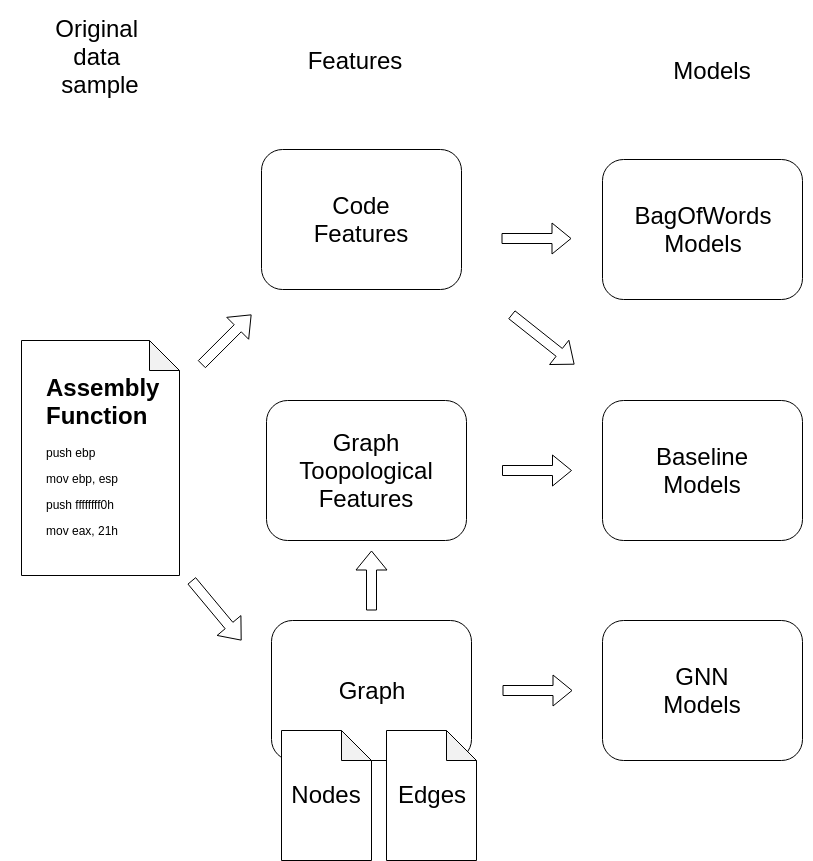
\includegraphics[width=0.65\linewidth]{img/Features_and_models_diagram.png}
    \caption{Features exracted from the dataset samples and their relationship with the models trained}\label{fig:Features_diagram}
\end{figure}



% function renaming experiments

% baseline models training (noisy,v1,v2,v3)
% nlp models training      (noisy,v1,v2,v3)
% gnn models training      (noisy,v1,v2,v3)




Building the dataset:
	- not any available dataset, -> selection of binaries + compilation with symbols 
	 + manual labelling
	labelling problem, choosing the correct granularity of the label (each binary a label= a lot of noise since all binaries have almost all functionalities implemented, topics=10 classes, topics-task but summarized=24 classes, fine grained topic-task=170 clases)
